\documentclass[a4paper, 12pt]{article}
\usepackage[utf8]{inputenc}
\usepackage[T1]{fontenc}
\usepackage[ngerman]{babel}
\usepackage{geometry}
\usepackage{listings}
\usepackage{xcolor}
\usepackage{hyperref}
\usepackage{helvet}
\usepackage{titlesec}
\usepackage{setspace}
\usepackage{graphicx}
\usepackage{pdfpages}
\usepackage{fancyhdr}
\usepackage{float}
\usepackage{enumitem}
\usepackage{tikz}
\usepackage{etoolbox}
\usepackage{tabularx}
\usepackage[style=apa, backend=biber, date=iso8601, urldate=iso8601]{biblatex}

\addbibresource{bibs/citavi.bib}

\DeclareFieldFormat{urldate}{
    Abgerufen am \thefield{urlday}\adddot\addspace\mkbibmonth{\thefield{urlmonth}}\addspace\thefield{urlyear} von
}

\hypersetup{breaklinks=true}

\definecolor{green}{HTML}{34A853}
\definecolor{orange}{HTML}{FBBC05}
\definecolor{red}{HTML}{EA4335}

\lstdefinelanguage{JavaScript}{
    keywords={break, case, catch, continue, debugger, default, delete, do, else, finally, for, function, if, in, instanceof, new, return, switch, this, throw, try, typeof, var, void, while, with},
    keywordstyle=\color{blue}\bfseries,
    ndkeywords={class, const, enum, export, extends, import, super, implements, interface, let, package, private, protected, public, static, yield, null, true, false},
    ndkeywordstyle=\color{darkgray}\bfseries,
    identifierstyle=\color{black},
    sensitive=false,
    comment=[l]{//},
    morecomment=[s]{/*}{*/},
    commentstyle=\color{purple}\ttfamily,
    stringstyle=\color{red}\ttfamily,
    morestring=[b]',
    morestring=[b]"
}

\lstset{
    language=JavaScript,
    extendedchars=true,
    basicstyle=\footnotesize\ttfamily,
    showstringspaces=false,
    showspaces=false,
    numbers=left,
    numberstyle=\footnotesize,
    numbersep=9pt,
    tabsize=2,
    breaklines=true,
    showtabs=false,
    captionpos=b
}
\geometry{a4paper, left=2.5cm, right=2.5cm, top=3cm, bottom=3cm, headsep=1.5cm}

\setlength{\parindent}{0pt}
\setlength{\parskip}{6pt}
\graphicspath{ {./images/} }

\pagestyle{fancy}
\fancyhf{}
\rhead{\vspace{0.2cm}
\includegraphics[width=4cm]{hs_mainz_logo}}
\fancypagestyle{plain}{
    \fancyhf{}
    \rhead{\vspace{0.2cm}
\includegraphics[width=4cm]{hs_mainz_logo}}
}
\renewcommand{\headrulewidth}{0pt}
\renewcommand{\footrulewidth}{0pt}
\fancyfoot[C]{\thepage}

\newcounter{lastroman}
\newrobustcmd{\switchtopage}[1]{
    \clearpage
    \setcounter{lastroman}{\value{page}}
    \pagenumbering{#1}
}
\newrobustcmd{\switchback}{
    \clearpage
    \pagenumbering{Roman}
    \setcounter{page}{\value{lastroman}}
}

% Document
\begin{document}

    \pagenumbering{Roman}

    \begin{titlepage}
    \centering
    \vspace*{1cm}

    
\includegraphics[width=0.4\textwidth]{hs_mainz_logo}\\
    \vspace{1.5cm}

    \textbf{\LARGE Praxismodul I}\\
    \vspace{0.5cm}
    \textbf{\Large Collectiqo}\\
    \vspace{1.5cm}

    \textbf{Hochschule Mainz}\\
    \vspace{0.5cm}
    Fachbereich Wirtschaft\\
    \vspace{0.5cm}
    B.Sc. Wirtschaftsinformatik dual\\
    \vspace{1.5cm}

    \textbf{Authors:}\\
    Bindernagel, Lorenz\\
    Schäfer, Robin\\
    Šimić, Darko\\
    Struve, Anika\\
    \vfill

    \today
\end{titlepage}
    \newpage

    \textbf{Nützliche Informationen:}\par
\vspace{0.5cm}
GitHub Repository: \url{https://github.com/LorackDev/collectiqo}\par
Datei für die Umgebungsvariablen ist nicht im Repository hinterlegt!\par
\vspace{0.5cm}
Dockerhub Hauptapplikation: \url{https://hub.docker.com/repository/docker/lorackdev/clq-app/general}\par
Dockerhub Custom MySQL: \url{https://hub.docker.com/repository/docker/lorackdev/clq-mysql/general}\par
Dockerhub Custom MongoDB: \url{https://hub.docker.com/repository/docker/lorackdev/clq-mongodb/general}\par
    \newpage

    \setcounter{page}{2}
    \tableofcontents
    \newpage

    \switchtopage{arabic}

    \section{Projektplanung- und Management}\label{sec:section-one}

Lorenz ipsum dolor sit amet, consetetur sadipscing elitr, sed diam nonumy eirmod tempor invidunt ut labore et dolore magna aliquyam erat, sed diam voluptua.
At vero eos et accusam et justo duo dolores et ea rebum.
Stet clita kasd gubergren, no sea takimata sanctus est Lorem ipsum dolor sit amet.
Lorenz ipsum dolor sit amet, consetetur sadipscing elitr, sed diam nonumy eirmod tempor invidunt ut labore et dolore magna aliquyam erat, sed diam voluptua.
At vero eos et accusam et justo duo dolores et ea rebum.
Stet clita kasd gubergren, no sea takimata sanctus est Lorem ipsum dolor sit amet.

\subsection{Rückblick auf Praxismodul I}\label{subsec:subsection-one-one}

Lorenz ipsum dolor sit amet, consetetur sadipscing elitr, sed diam nonumy eirmod tempor invidunt ut labore et dolore magna aliquyam erat, sed diam voluptua.
At vero eos et accusam et justo duo dolores et ea rebum.
Stet clita kasd gubergren, no sea takimata sanctus est Lorem ipsum dolor sit amet.
Lorenz ipsum dolor sit amet, consetetur sadipscing elitr, sed diam nonumy eirmod tempor invidunt ut labore et dolore magna aliquyam erat, sed diam voluptua.
At vero eos et accusam et justo duo dolores et ea rebum.
Stet clita kasd gubergren, no sea takimata sanctus est Lorem ipsum dolor sit amet.

\subsection{Zielsetzungen im Praxismodul II}\label{subsec:subsection-one-two}

Lorenz ipsum dolor sit amet, consetetur sadipscing elitr, sed diam nonumy eirmod tempor invidunt ut labore et dolore magna aliquyam erat, sed diam voluptua.
At vero eos et accusam et justo duo dolores et ea rebum.
Stet clita kasd gubergren, no sea takimata sanctus est Lorem ipsum dolor sit amet.
Lorenz ipsum dolor sit amet, consetetur sadipscing elitr, sed diam nonumy eirmod tempor invidunt ut labore et dolore magna aliquyam erat, sed diam voluptua.
At vero eos et accusam et justo duo dolores et ea rebum.
Stet clita kasd gubergren, no sea takimata sanctus est Lorem ipsum dolor sit amet.

\subsection{Projektorganisationen}\label{subsec:subsection-one-three}

Lorenz ipsum dolor sit amet, consetetur sadipscing elitr, sed diam nonumy eirmod tempor invidunt ut labore et dolore magna aliquyam erat, sed diam voluptua.
At vero eos et accusam et justo duo dolores et ea rebum.
Stet clita kasd gubergren, no sea takimata sanctus est Lorem ipsum dolor sit amet.
Lorenz ipsum dolor sit amet, consetetur sadipscing elitr, sed diam nonumy eirmod tempor invidunt ut labore et dolore magna aliquyam erat, sed diam voluptua.
At vero eos et accusam et justo duo dolores et ea rebum.
Stet clita kasd gubergren, no sea takimata sanctus est Lorem ipsum dolor sit amet.

\subsection{Tools}\label{subsec:subsection-one-four}

Lorenz ipsum dolor sit amet, consetetur sadipscing elitr, sed diam nonumy eirmod tempor invidunt ut labore et dolore magna aliquyam erat, sed diam voluptua.
At vero eos et accusam et justo duo dolores et ea rebum.
Stet clita kasd gubergren, no sea takimata sanctus est Lorem ipsum dolor sit amet.
Lorenz ipsum dolor sit amet, consetetur sadipscing elitr, sed diam nonumy eirmod tempor invidunt ut labore et dolore magna aliquyam erat, sed diam voluptua.
At vero eos et accusam et justo duo dolores et ea rebum.
Stet clita kasd gubergren, no sea takimata sanctus est Lorem ipsum dolor sit amet.
    \newpage

    \subsection{Reorganisation der Projektstruktur}\label{subsec:subsection-two-one}

Das vorherige Semester war das erste Mal, dass das Team eine Node JS Applikation entwickelt hat.
Demnach wurde viel ausprobiert und es war noch kein Verständnis darüber vorhanden, wie eine solche Anwendung gut strukturiert aufgebaut wird.
Dieses Verständnis wurde über das letzte Semester aufgebaut und es wurde beschlossen, das Projekt neu zu strukturieren.
Dies kostete zum Anfang des Semesters viel Zeit, hat jedoch den Effekt, dass eine einheitliche Struktur aufgebaut wurde und die Implementierung neuer Funktionen einfach sind und einem fest definierten Standard folgen.

\subsubsection{Struktur des Projektstammverzeichnis}
Im ersten Abschnitt wird auf die Gliederung in der ersten Ebene der Projektstruktur eingegangen, dem Projektstammverzeichnis.
Während im vorherigen Semester eine Funktion meist alle Komponenten, wie Responses und die eigentliche Funktionalität in einer Datei beinhalteten, wurden diese Dateien nun in drei einzelne Dateien aufgeteilt.
Zuvor wurden alle Routen einzeln in der app.js Datei definiert, welches die Datei sehr aufblähte.
In der app.js wird in der neuen Version eine Route Loader Funktion aufgerufen, die dynamisch alle definierten Routen im Projekt erkennt und hinzufügt.

Um die neue Idee umzusetzen wurden alle Ordner und Dateien, die den eigentlichen Programmcode beinhalten, in einen Ordner namens \textit{src} abgelegt.
Dies hilft auch beim Bauen des Docker Images, da nun in der Dockerfile nur die Inhalte des src Ordners kopiert werden.
So wird kein unnötiger und ungewollter Overhead an Dateien in das Docker Image eingebaut.
Dateien wie \textit{.env}, die \textit{docker-compose.yaml} sowie der \textit{node\_modules} Ordner gehören nicht mit in das Image, da sie unter anderem sensible Daten beinhalten, die jeder mit Zugriff auf das Docker Image einsehen kann.
Hier ist ein Vergleich der Projektstruktur nach dem letzten Commit des ersten Praxismoduls vs nach der Umstrukturierung in diesem Praxismodul:
\begin{figure}[h]
  \centering
  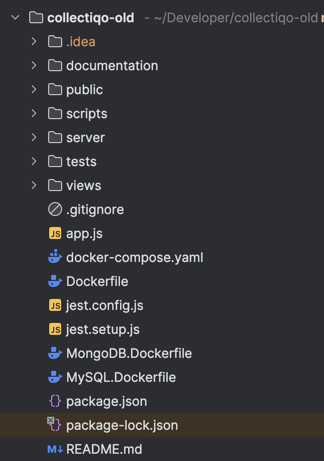
\includegraphics[width=0.3\textwidth]{root_path_structure_old}
  \caption{Alte Projektstruktur}
  \label{fig:root_path_structure_old}
\end{figure}

\newpage

\begin{figure}[h]
  \centering
  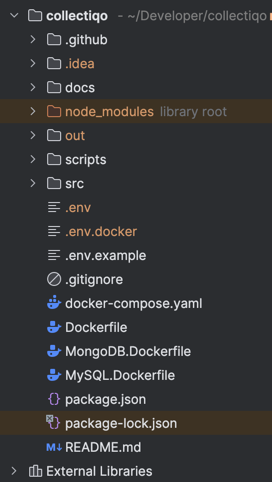
\includegraphics[width=0.3\textwidth]{root_path_structure_new}
  \caption{Neue Projektstruktur}
  \label{fig:root_path_strucutr_new}
\end{figure}
Code, der zuvor unter den Ordnern Server, Public und Views zu finden war, wurde nun in den src Ordner verlagert.
Die gesamte Projektstruktur ist auf der \href{https://github.com/LorackDev/collectiqo}{Collectiqo Github Seite} einsehbar.
Im nächsten Abschnitt wird der Inhalt des src Ordners genauer betrachtet.

\subsubsection{Struktur des Quellcodes}
Wie zuvor beschrieben beinhaltet der src Ordner jegliche Dateien, die den Quellcode der Collectiqo App beinhalten.
Hierzu zählen ebenfalls einige Ordner wie der public und views Ordner, die zuvor auf root Ebene vorhanden waren.
Hier eine Übersicht über alle Inhalte des neuen src Ordners:
\begin{figure}[h]
  \centering
  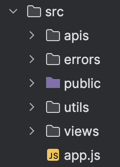
\includegraphics[width=0.3\textwidth]{src_folder_structure}
  \caption{src Ordner Struktur}
  \label{fig:src_folder_structure}
\end{figure}

\newpage

Während zuvor alle Bestandteile einer Funktion (Route, Response Codes und Funktionalität) in einer Datei gehandhabt wurden, wurden diese nun in drei separate Dateien aufgeteilt.
Jede Route erhält eine eigene Datei, in welcher der Endpunkt für HTTP Request definiert wird und der entsprechende Controller aufgerufen wird.
Hier ein Beispiel für die Route der Login Funktion:

\vspace{1em}
\lstset{language=javascript}
\begin{lstlisting}[label={lst:lst-login-route}]
const express = require('express');
const router = express.Router();
const loginController = require('../controllers/loginController');

router.post('/login', loginController);

module.exports = router;
\end{lstlisting}
\vspace{1em}


Der Controller kümmert sich um den Aufruf der gewünschten Service Datei und handhabt die Response Codes, die beim Aufruf des Endpunkts zurückgegeben werden.
Als Beispiel dient dieser Controller der Login Funktion:

\vspace{1em}
\begin{lstlisting}[label={lst:lst-login-controller}]
const loginService = require('../services/loginService');

// Extract constants for response messages
const LOGIN_SUCCESS_MESSAGE = 'Login successful';
const INTERNAL_SERVER_ERROR_MESSAGE = 'Internal server error';

// Extract error handling into a separate function
const handleLoginError = (res, error) => {
  console.error('Login error:', error);
  res.status(500).json({message: INTERNAL_SERVER_ERROR_MESSAGE});
};

const loginController = async (req, res) => {
  const {username, password} = req.body;
  try {
    // check if user can be found in database
    const user = await loginService(username, password);
    // throw error if user can't be found
    if(user===undefined){
      throw new Error('User not found')
    }
    // add user data to session variables
    req.session.user = {
      name: user.username,
      id: user.id,
      isLoggedIn: true
    }

    // try to save changes, else throw error
    try {
      await req.session.save();
      console.log(`User ${req.session.user.name} logged in successfully`);
      res.status(200).json({message: LOGIN_SUCCESS_MESSAGE, userId: req.session.user.id});
    } catch (err) {
      console.error('Error saving to session storage: ', err);
      return new Error('Error logging in user');
    }
  } catch (error) {
    handleLoginError(res, error);
  }
};

module.exports = loginController;
\end{lstlisting}
\vspace{1em}

Die eigentliche Funktionalität ist in der Service Datei implementiert.
Zuletzt noch die Service Datei der Login Funktion:

\vspace{1em}
\begin{lstlisting}[label={lst:lst-login-service}]
const bcrypt = require('bcryptjs');
const { queryDatabase, handleResults } = require('../../../utils/mysqlUtils');

const loginService = async (username, password) => {
    const results = await queryDatabase('SELECT * FROM clq_users WHERE username = ? OR email = ?', [username, username]);
    const user = handleResults(results);

    if (!user) {
        throw new Error('User not found');
    }

    const passwordMatches = await bcrypt.compare(password, user.password);
    if (!passwordMatches) {
        throw new Error('Incorrect password');
    }

    return user; // Ensure the user object is returned
};

module.exports = loginService;
\end{lstlisting}
\vspace{1em}

Diese Aufteilung bringt mehrere Vorteile mit sich.
Jede Funktionalität, die ab sofort implementiert wird, folgt genau diesem Muster, wodurch jede Implementierung für jedes Teammitglied klar nachverfolgbar ist.
Darüber hinaus erleichtert es das Debugging ungemein, da Probleme einfacher auf einzelne Bestandteile eines Funktionsaufrufs zurückgeführt werden können.
Kombiniert mit einer Ordnerstruktur, die inhaltlich ferne Funktionen voneinander trennt, ist auf das Navigieren innerhalb des Projekts vereinfacht.
Schlussendlich ist auch das Aufrufen vom HTTP Requests vereinfacht, da jeder Aufruf einheitlich ist.
    \newpage

    \section{Designanalyse}\label{sec:section-three}

Zu Beginn der Projektarbeit wurde eine umfassende Designanalyse durchgeführt und sorgfältig dokumentiert.
Im Rahmen dieser Analyse wurden verschiedene zentrale Bestandteile des bestehenden Designs betrachtet, darunter die Loginpage, die Landingpage, die Sidebar, Menüs, die Collectionseite einschließlich der Ansicht einzelner Kollektionen sowie die Accounteinstellungen.

Auffällig war insbesondere die Farbpalette des bisherigen Designs.
Obwohl ursprünglich mit einem festgelegten Farbschema gearbeitet wurde, konnten Abweichungen festgestellt werden.
Diese Abweichungen sind größtenteils auf Zeitmangel während der Umsetzung des vorherigen Projekts zurückzuführen.

Des Weiteren wurde festgestellt, dass für das bisherige Design generierte Bilder verwendet wurden.
Diese sollen unverändert erhalten bleiben, da sie gut zum Gesamtkonzept passen.
Zur Veranschaulichung der Startseite wurde außerdem ein Photoshop-Mockup erstellt, welches als erste Orientierung für die Überarbeitung des Designs dient.

Für jede wesentliche Seite des Projekts wurde anschließend eine gezielte Designrecherche betrieben.
Im Zuge dieser Recherche zeigte sich, dass bestimmte gestalterische Ähnlichkeiten zwischen den untersuchten Designs bestehen, die wir als Inspirationsquelle nutzen und bewusst in unser überarbeitetes Design integrieren möchten.

\subsection{Rechtliche Vorgaben}\label{subsec:subsection-three-one}

Bei der Gestaltung von Webseiten sind neben ästhetischen und funktionalen Aspekten auch rechtliche Vorgaben zu beachten.
Eine der zentralen Vorgaben ist die Einhaltung der Datenschutz-Grundverordnung (DSGVO).
Webseiten müssen transparent über die Erhebung und Verarbeitung personenbezogener Daten informieren.
Dazu gehören eine gut zugängliche Datenschutzerklärung sowie ein Cookie-Banner, das Nutzern die Möglichkeit gibt, der Nutzung von Cookies aktiv zuzustimmen oder sie abzulehnen.

Zusätzlich ist das Telemediengesetz (TMG) relevant, das unter anderem die Pflicht zur Bereitstellung eines Impressums regelt.
Dieses muss auf der Webseite leicht auffindbar sein und vollständige Angaben zu Verantwortlichen und Kontaktmöglichkeiten enthalten.

Ein weiterer wichtiger Aspekt ist die Barrierefreiheit, insbesondere für öffentliche Institutionen, die durch die EU-Richtlinie 2016/2102 verpflichtet sind, ihre Webseiten barrierefrei zu gestalten.
Dazu gehört die Bereitstellung von alternativen Texten für Bilder, eine intuitive Navigation und eine klare, kontrastreiche Gestaltung.
Dieses wurde aufgrund der Eingrenzung als bisher nicht-öffentliches Universitätsprojekt vorerst nicht beachtet.

\parencite{GIDF.2024}
% TODO: Just for Testing, you know! ;)

\subsection{Visuelles Redesign}\label{subsec:subsection-three-two}

Im Rahmen des Redesigns wurden zentrale Änderungen vorgenommen, um das bestehende Design zu modernisieren, benutzerfreundlicher zu gestalten und zu vereinheitlichen.
Eine der ersten Maßnahmen war die Anpassung der Farbpalette, die vollständig auf harmonische Lilatöne umgestellt wurde.
Dies erlaubt für eine potentielle Einführung eines Dunkel-Hell Modi und bietet eine bessere Ästhetik hinblickend auf die Philosophie von Collectiqo.

Alte Seiten, die zuvor den Designcode gebrochen hatten, wurden überarbeitet, um eine einheitliche visuelle Sprache sicherzustellen.
Zusätzlich wurde ein modernes, rundes Theme eingeführt, das die Benutzeroberfläche klarer und ansprechender macht.
Dies ist insbesondere beim Erstellen von Collections und der Accounteinstellungen einzusehen.

Ein wichtiger Schritt im Redesign war die Zusammenlegung und Komprimierung verschiedener Seiten.
Es wurde die Startseite mit dem Sign-Up verknüpft, und die Accounteinstellungen wurden in verschiedene Reiter gelegt.
Dadurch wurde die Benutzerführung vereinfacht und die Navigation für neue Nutzer intuitiver gestaltet.

Zur Verbesserung der Interaktion wurden Übergänge zwischen den Seiten implementiert, die das Nutzungserlebnis flüssiger gestalten sollen.
Allerdings lief die Umsetzung dieser Übergänge nicht immer optimal, was als zukünftiger Optimierungsbereich identifiziert wurde.
    \newpage

    \section{Technische Implementierung}\label{sec:section-four}

Lorenz ipsum dolor sit amet, consetetur sadipscing elitr, sed diam nonumy eirmod tempor invidunt ut labore et dolore magna aliquyam erat, sed diam voluptua.
At vero eos et accusam et justo duo dolores et ea rebum.
Stet clita kasd gubergren, no sea takimata sanctus est Lorem ipsum dolor sit amet.
Lorenz ipsum dolor sit amet, consetetur sadipscing elitr, sed diam nonumy eirmod tempor invidunt ut labore et dolore magna aliquyam erat, sed diam voluptua.
At vero eos et accusam et justo duo dolores et ea rebum.
Stet clita kasd gubergren, no sea takimata sanctus est Lorem ipsum dolor sit amet.

\subsection{Webfrontend}\label{subsec:subsection-four-one}

Lorenz ipsum dolor sit amet, consetetur sadipscing elitr, sed diam nonumy eirmod tempor invidunt ut labore et dolore magna aliquyam erat, sed diam voluptua.
At vero eos et accusam et justo duo dolores et ea rebum.
Stet clita kasd gubergren, no sea takimata sanctus est Lorem ipsum dolor sit amet.
Lorenz ipsum dolor sit amet, consetetur sadipscing elitr, sed diam nonumy eirmod tempor invidunt ut labore et dolore magna aliquyam erat, sed diam voluptua.
At vero eos et accusam et justo duo dolores et ea rebum.
Stet clita kasd gubergren, no sea takimata sanctus est Lorem ipsum dolor sit amet.

\subsection{Backend}\label{subsec:subsection-four-two}

Lorenz ipsum dolor sit amet, consetetur sadipscing elitr, sed diam nonumy eirmod tempor invidunt ut labore et dolore magna aliquyam erat, sed diam voluptua.
At vero eos et accusam et justo duo dolores et ea rebum.
Stet clita kasd gubergren, no sea takimata sanctus est Lorem ipsum dolor sit amet.
Lorenz ipsum dolor sit amet, consetetur sadipscing elitr, sed diam nonumy eirmod tempor invidunt ut labore et dolore magna aliquyam erat, sed diam voluptua.
At vero eos et accusam et justo duo dolores et ea rebum.
Stet clita kasd gubergren, no sea takimata sanctus est Lorem ipsum dolor sit amet.

\subsection{Datenbank}\label{subsec:subsection-four-tree}

Lorenz ipsum dolor sit amet, consetetur sadipscing elitr, sed diam nonumy eirmod tempor invidunt ut labore et dolore magna aliquyam erat, sed diam voluptua.
At vero eos et accusam et justo duo dolores et ea rebum.
Stet clita kasd gubergren, no sea takimata sanctus est Lorem ipsum dolor sit amet.
Lorenz ipsum dolor sit amet, consetetur sadipscing elitr, sed diam nonumy eirmod tempor invidunt ut labore et dolore magna aliquyam erat, sed diam voluptua.
At vero eos et accusam et justo duo dolores et ea rebum.
Stet clita kasd gubergren, no sea takimata sanctus est Lorem ipsum dolor sit amet.
    \newpage

    \section{Funktionserweiterungen}\label{sec:section-five}

Lorenz ipsum dolor sit amet, consetetur sadipscing elitr, sed diam nonumy eirmod tempor invidunt ut labore et dolore magna aliquyam erat, sed diam voluptua.
At vero eos et accusam et justo duo dolores et ea rebum.
Stet clita kasd gubergren, no sea takimata sanctus est Lorem ipsum dolor sit amet.
Lorenz ipsum dolor sit amet, consetetur sadipscing elitr, sed diam nonumy eirmod tempor invidunt ut labore et dolore magna aliquyam erat, sed diam voluptua.
At vero eos et accusam et justo duo dolores et ea rebum.
Stet clita kasd gubergren, no sea takimata sanctus est Lorem ipsum dolor sit amet.

\subsection{Integrationstests}\label{subsec:subsection-five-one}

Lorenz ipsum dolor sit amet, consetetur sadipscing elitr, sed diam nonumy eirmod tempor invidunt ut labore et dolore magna aliquyam erat, sed diam voluptua.
At vero eos et accusam et justo duo dolores et ea rebum.
Stet clita kasd gubergren, no sea takimata sanctus est Lorem ipsum dolor sit amet.
Lorenz ipsum dolor sit amet, consetetur sadipscing elitr, sed diam nonumy eirmod tempor invidunt ut labore et dolore magna aliquyam erat, sed diam voluptua.
At vero eos et accusam et justo duo dolores et ea rebum.
Stet clita kasd gubergren, no sea takimata sanctus est Lorem ipsum dolor sit amet.

\subsection{Teilen-Funktion???}\label{subsec:subsection-five-two}

Lorenz ipsum dolor sit amet, consetetur sadipscing elitr, sed diam nonumy eirmod tempor invidunt ut labore et dolore magna aliquyam erat, sed diam voluptua.
At vero eos et accusam et justo duo dolores et ea rebum.
Stet clita kasd gubergren, no sea takimata sanctus est Lorem ipsum dolor sit amet.
Lorenz ipsum dolor sit amet, consetetur sadipscing elitr, sed diam nonumy eirmod tempor invidunt ut labore et dolore magna aliquyam erat, sed diam voluptua.
At vero eos et accusam et justo duo dolores et ea rebum.
Stet clita kasd gubergren, no sea takimata sanctus est Lorem ipsum dolor sit amet.
    \newpage

    \section{Fazit und Ausblick}\label{sec:fazit-ausblick}

Dieses Kapitel fasst die wichtigsten Erkenntnisse zusammen, beleuchtet Abweichungen von den ursprünglichen Zielen und reflektiert die Fortschritte des Projekts.
Gleichzeitig wird ein Ausblick auf zukünftige Schritte gegeben, um das Projekt weiterzuentwickeln und an neue Herausforderungen anzupassen.

\subsection{Abweichungen der geplanten Ziele}\label{subsec:abweichungen-der-geplanten-ziele}

Im Rahmen des Projekts konnten einige der gesetzten Ziele erfolgreich umgesetzt werden, während andere aufgrund unvorhergesehener Herausforderungen nicht erreicht wurden.

\begin{itemize}[noitemsep]
    \item \textbf{Restrukturierung der GitHub-Struktur}: Dieses Ziel wurde vollständig erreicht, wodurch eine klarere Organisation und Nachvollziehbarkeit des Projekts gewährleistet ist.
    \item \textbf{Auslagerung von redundanten Code-Snippets in HTML, CSS und JavaScript}: Die Reduktion von Redundanzen wurde erfolgreich umgesetzt, was die Wartbarkeit und Skalierbarkeit des Projekts deutlich verbessert hat.
    \item \textbf{Designanpassung mit richtigem Branding}: Das Branding wurde erfolgreich implementiert, was zu einem professionelleren und kohärenten Auftritt beiträgt.
    \item \textbf{Projektmanagement-Tool}: Der Wechsel auf ein neues Projektmanagement-Tool konnte zu Beginn des Praxismoduls II erfolgreich umgesetzt werden, was die Organisation und Kommunikation im Team verbessert hat.
    \item \textbf{Docker-Erweiterung}: Die Docker-Umgebung konnte erfolgreich um zwei Container (Reverse Proxy und Certbot Zertifikatsverwaltung) erweitert werden.
    \item \textbf{Bugs im Front- und Backend}: Die Behebung von Bugs wurde erfolgreich durchgeführt, was die Stabilität und Zuverlässigkeit der Plattform erhöht hat.
    \item \textbf{vServer-Hosting}: Die Plattform konnte erfolgreich auf einem vServer gehostet werden, was die Verfügbarkeit verbessert und die Grundlage für zukünftige Erweiterungen schafft.
    \item \textbf{DB-Constrains}: Die Absicherung der Datenbank durch Constraints konnte aus Zeitgründen nicht umgesetzt werden, bleibt aber ein Ziel für zukünftige Entwicklungen.
    \item \textbf{Integrationstests}: Die Implementierung von Integrationstests konnte ebenfalls nicht umgesetzt werden und verbleibt im Backlog.
    \item \textbf{Erweiterung der Funktionen für die Anpassung von Collections}: Dieses Ziel konnte nicht erreicht werden, da die notwendigen Umstrukturierungen und die Vereinheitlichung anderer Komponenten mehr Zeit in Anspruch nahmen als ursprünglich geplant.
\end{itemize}

\newpage

\subsection{Retrospektive}\label{subsec:retrospektive}

Im Vergleich zum ersten Semester haben wir uns bewusst weniger vorgenommen, um einen klaren Fokus auf die grundlegende Restrukturierung des Projektes zu legen.
Unser Hauptziel war es, die Wiederverwendbarkeit von Code zu ermöglichen und damit eine nachhaltige Grundlage für zukünftige Entwicklungen zu schaffen.
Die Teammitglieder konnten zudem gezielter persönlichen Interessen nachgehen und sich in spezifischen Bereichen vertiefen.

Ein weiterer Schwerpunkt lag auf der Verbesserung der Benutzerfreundlichkeit und der Gestaltung ansprechender Designs.
Diese Maßnahmen sollten sicherstellen, dass spätere Funktionserweiterungen ohne größere Rückschritte oder grundlegende Änderungen umgesetzt werden können.

Durch diese gezielte Herangehensweise haben wir eine solide Basis geschaffen, die sowohl die technische als auch die visuelle Qualität des Projekts langfristig unterstützt.

\subsection{Ausblick}\label{subsec:ausblick-zukuenftige-ziele-und-funktionen}

Das Projektteam strebt an, die Plattform \textbf{Collectiqo} auch im Praxismodul III weiterzuentwickeln und zu verbessern.
Zukünftig sind weitere Erweiterungen und Verbesserungen geplant, um die Funktionalität bzw. Sicherheit der Plattform zu steigern und auszubauen.
Dazu gehören nach aktuellem Stand überlegungen in Richtung:

\begin{itemize}[noitemsep]
    \item Vollständige Collectionansicht mit Bearbeitung der Collections.
    \item Änderbare Einstellungen der Benutzerdaten durch User selbst.
    \item Ausbau der vServer-Infrastruktur, Optimierung und Fortentwicklung von Funktionalitäten.
    \item Betrachtung der Anmeldung einer Wortmarke für rechtlichen Schutz.
    \item Implementierung eines E-Mail-Bestätigungscodes für die Registrierung sowie eine „Passwort vergessen“-Funktion.
    \item Verteiltes Arbeiten an der Plattform in dedizierten branches.
    \item Pipelines für Auto-Deployment auf dem vServer.
\end{itemize}



    \newpage

    \pagenumbering{roman}
    \setcounter{page}{1}

    \printbibliography

\end{document}